\chapter{Perancangan dan Relasi Antar Tabel}

\section{Perancangan Tabel}
Pada bagian ini kita membuat perancangan tabel sebagai berikut : 
\begin{figure}[H]
	\centering
	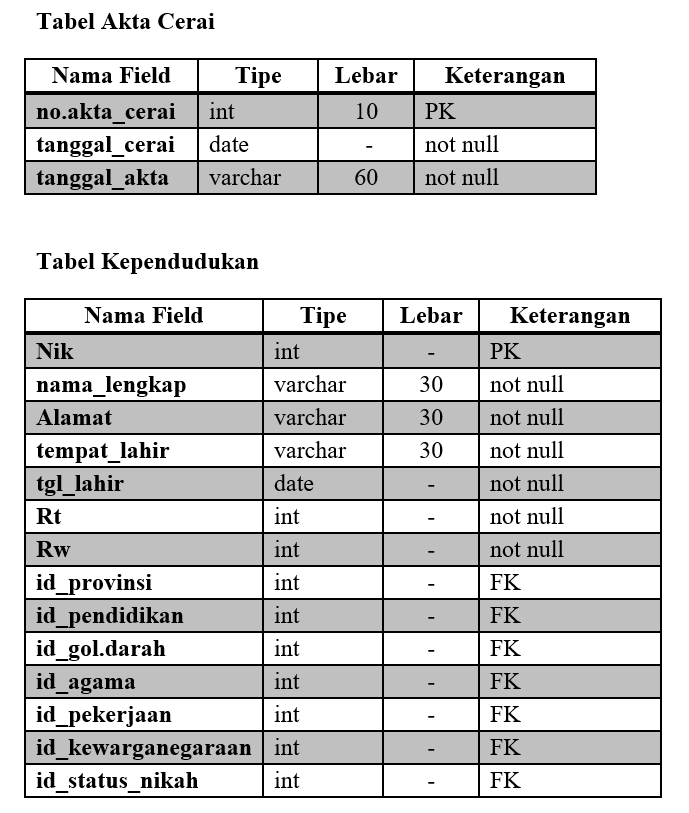
\includegraphics[width=10cm]{figures/tabel1.png}
\end{figure}
\begin{figure}[H]
	\centering
	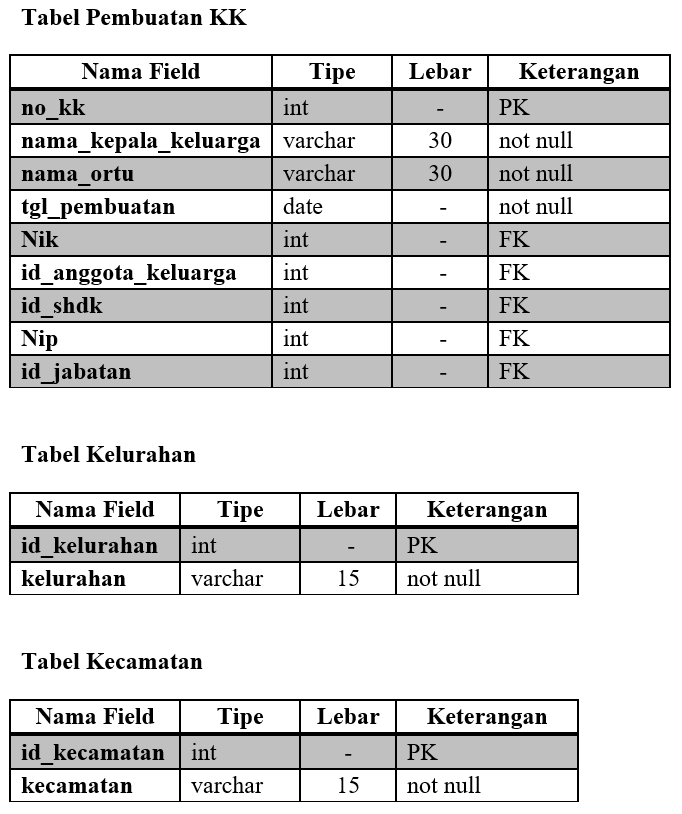
\includegraphics[width=8cm]{figures/tabel2.png}
\end{figure}
\begin{figure}[H]
	\centering
	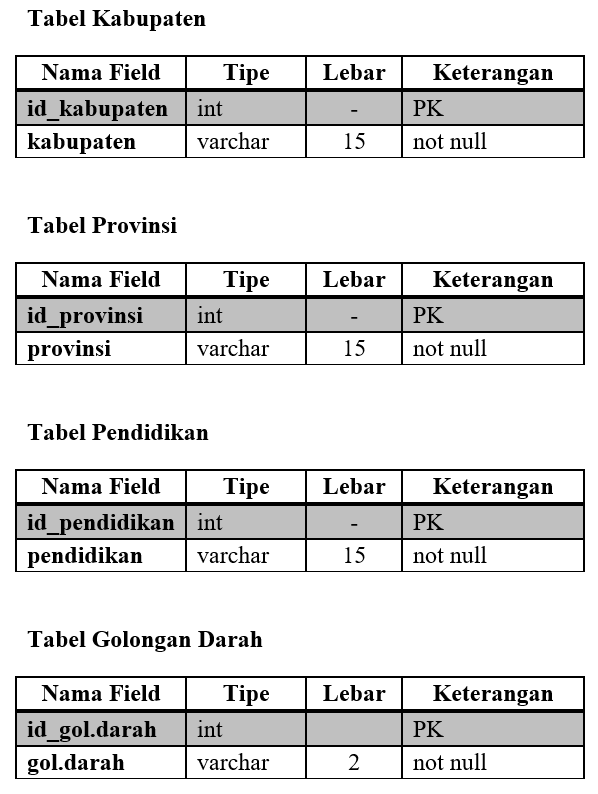
\includegraphics[width=8cm]{figures/tabel3.png}
\end{figure}
\begin{figure}[H]
	\centering
	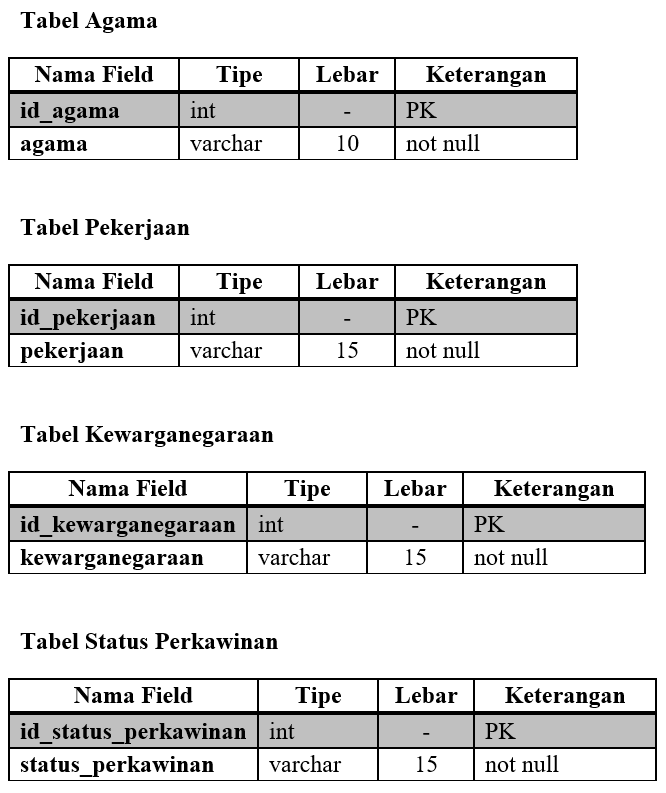
\includegraphics[width=8cm]{figures/tabel4.png}
\end{figure}
\begin{figure}[H]
	\centering
	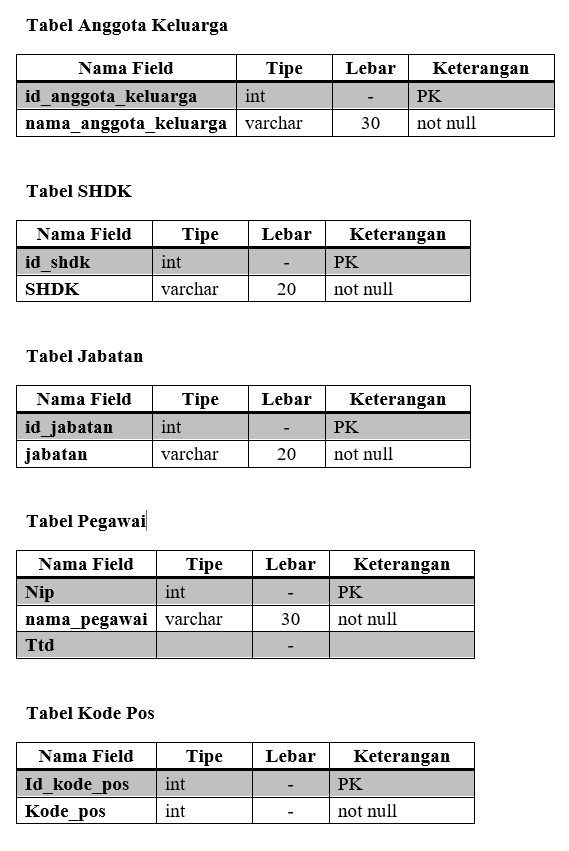
\includegraphics[width=8cm]{figures/tabel5.png}
\end{figure}
\section{Relasi Database KK Perceraian}
\begin{figure}[H]
	\centering
	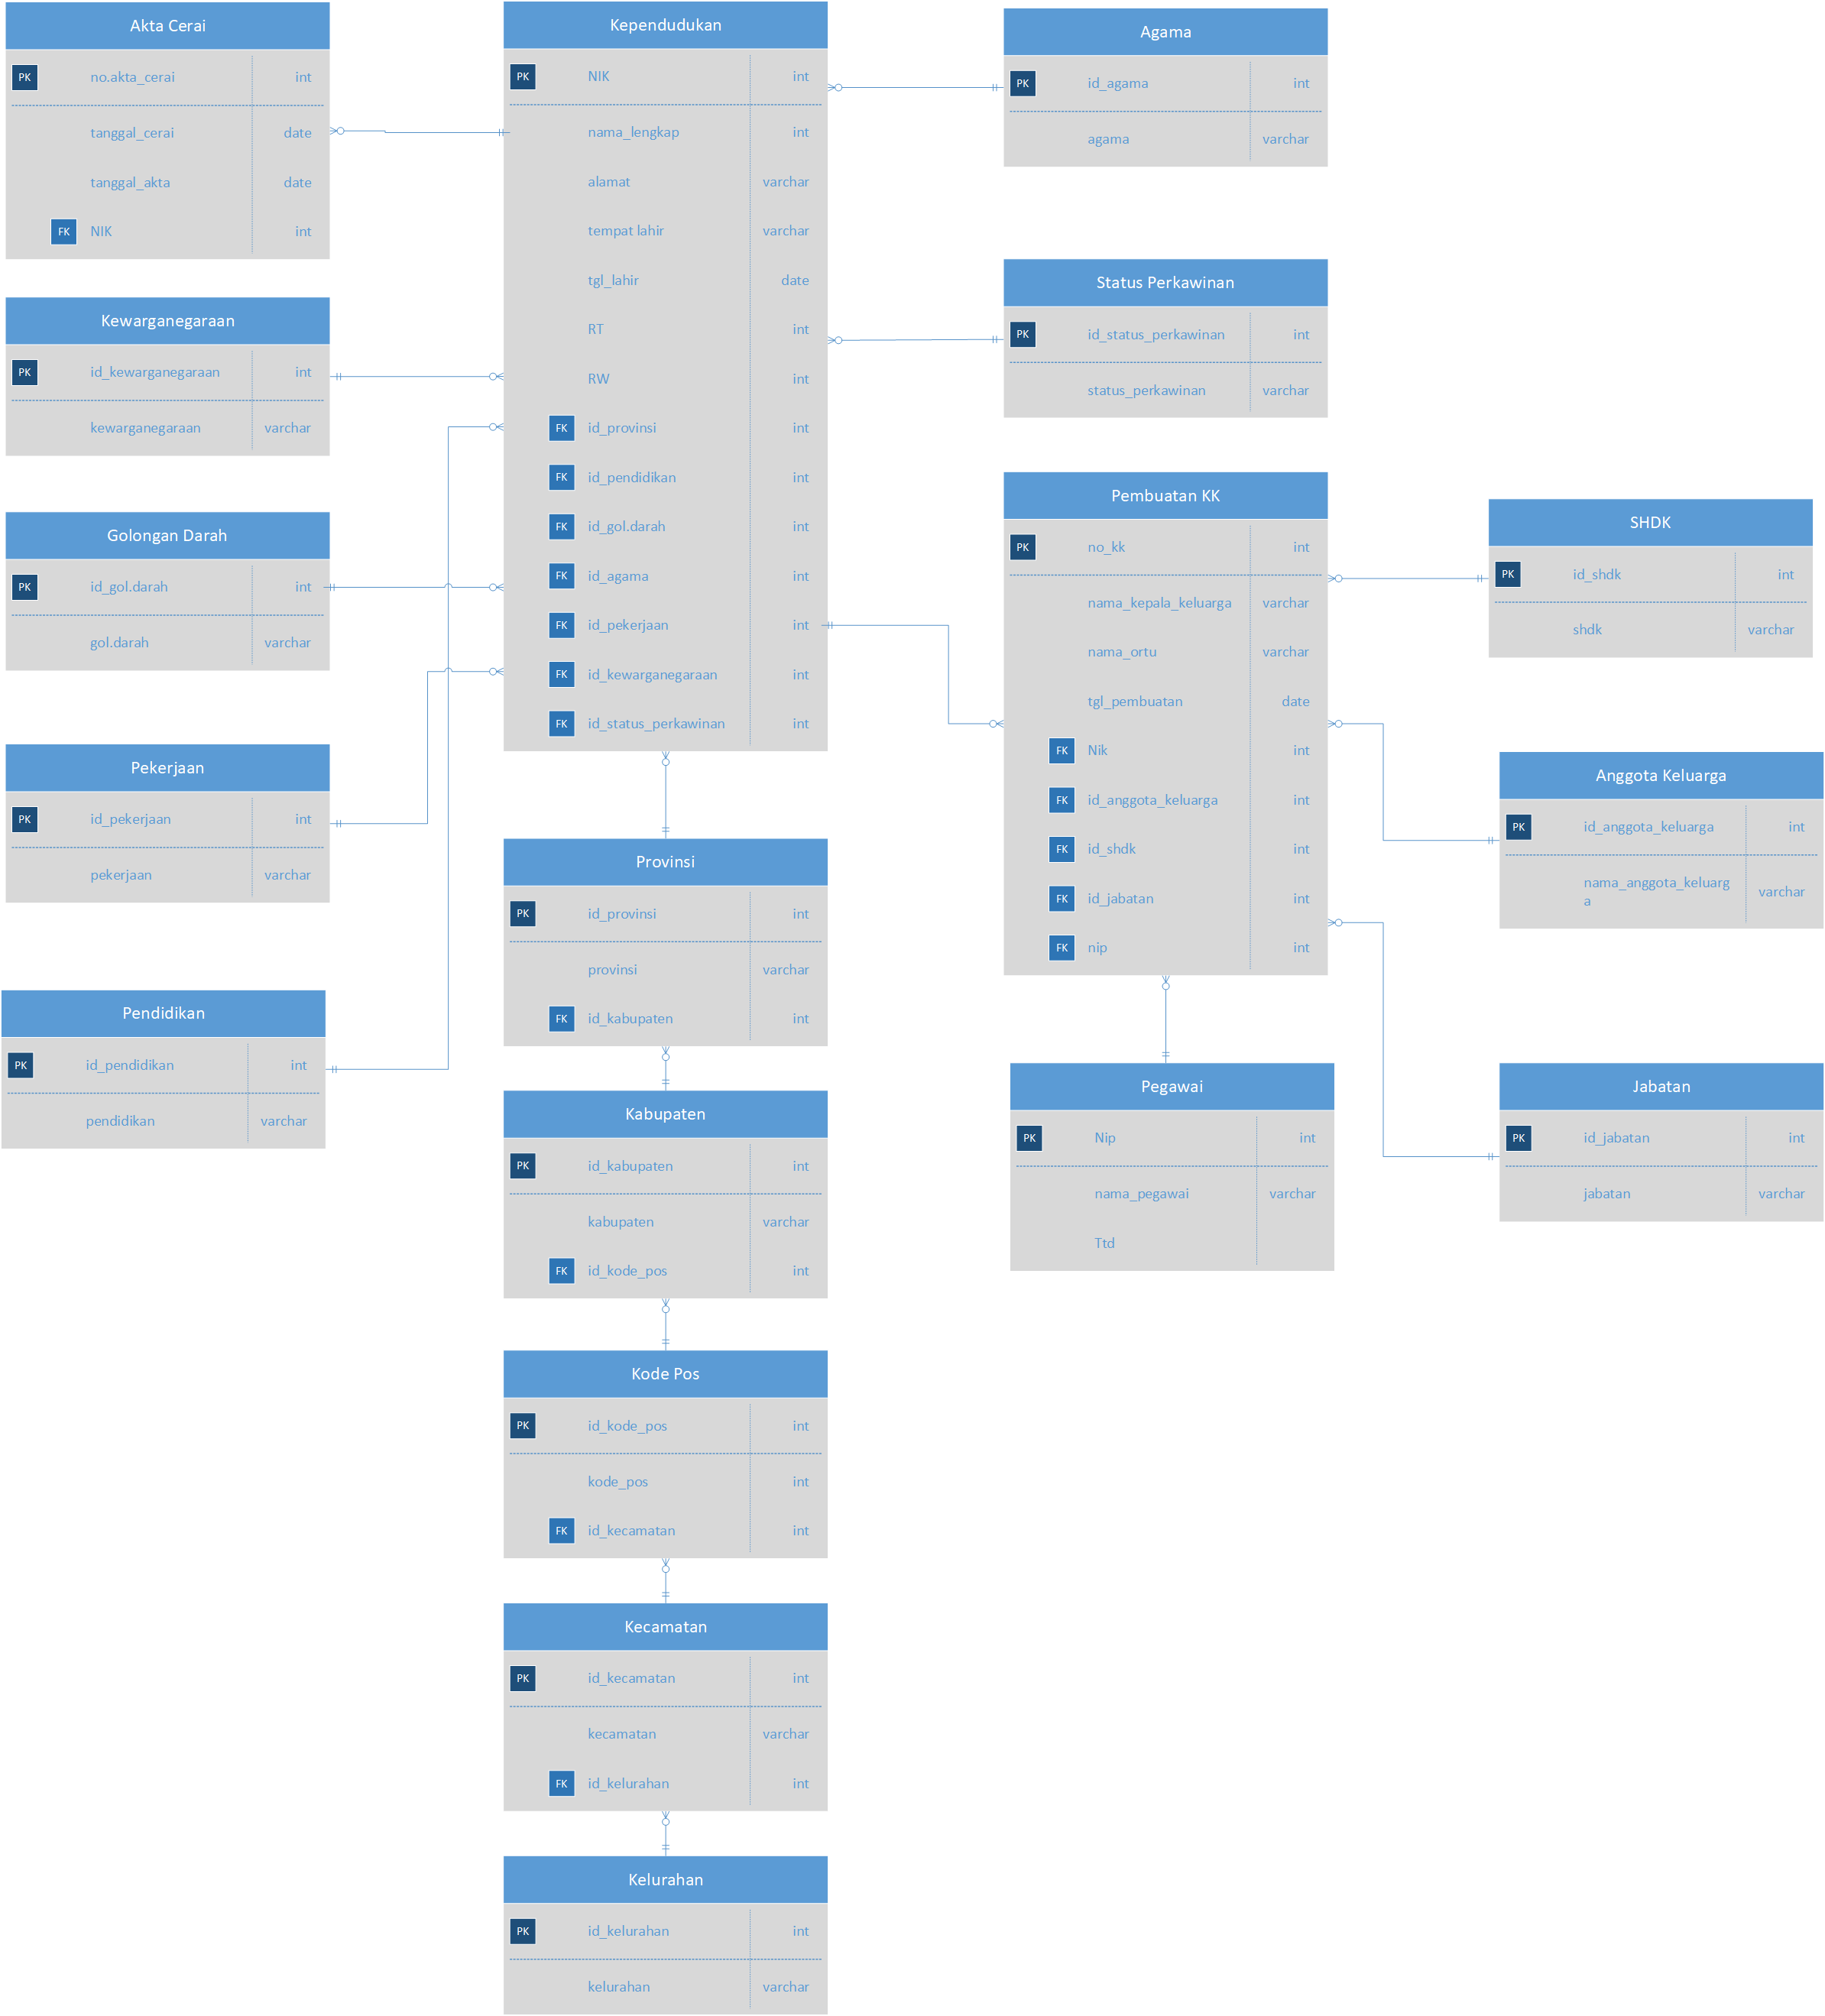
\includegraphics[width=14cm]{figures/relasi.png}
	\caption{Tabel Database Perancangan dan Relasi KK Perceraian.}
\end{figure}
